\documentclass{article}
\usepackage{amsthm}
\usepackage{graphicx}

\linespread{2}

\author{Eric Bauerfeld}
\title{Simulating the Spread of Tweets via Naive Bayesian Classifiers}

\begin{document}

\maketitle

\newpage

\section{Introduction}

Social media networks are an increasingly important technology. In order to effectively use these networks for marketing or spreading news, being able to predict the spread of information by anticipating the effectiveness of particular wordings would be quite useful. This paper will explore how one could simulate a twitter network and use the network's prior history of communication to determine whether a tweet is likely to be retweeted and how far it is likely to spread within that network. We will do so via the use of Naive Bayesian Classifiers.

\section{Assumptions}

Our model is quite simple, and is making a number of assumptions about the nature of our data. Our first major assumption is that text content is the only significant factor when a user decides to retweet something. This assumption was made in order to simplify our decision making criteria for the spread of a new tweet, and to allow us to more easily predict whether a tweet is likely to be sent with minimal assumptions about the context. This means we are assuming that the text content is more important that the originating user, the content of images/videos/other links, the time at which the tweet was made, and the amount of favorites or retweets at the time the tweet was viewed.

In order to classify whether words are likely to be retweeted, we needed to collect all of the tweets that were visible to each user in our network. When doing this, we assumed that the only candidates for retweets are from users the current user in question is following, and treated all tweets as equally visible to the user.

We are also implicitly assuming that the words within a sentence are independent of each other, as Naive Bayesian Classifiers assume the occurrences being measured are independent. Although this is not the case with the English language, this approach has been used in other contexts with surprisingly accurate results, so we are considering it adequate for our purposes.

\section{Model}

First, we constructed a network of 20 users. This network was obtained via a python script that looked at the users a particular user was following. In order to make our network interesting looking, the code was written so that we'd get all the users a particular user was following, then select 3 users from that list, then get all of the users they were following, then repeat until we had 20 users, plus all the users those 20 users were following. For each user a member of our network was following, we downloaded their entire history of tweets.

After those tweets were downloaded, we broke down the tweets into individual tokens, which in this case were words. For each user, we then counted the total number of retweets, which we assigned a positive classification class, the total number of tweets not retweeted, which we assigned a negative classification class, and the total number of tweets. We then classified the occurrences of each specific word per user and counted occurrences in tweets retweeted, occurrences in tweets not retweeted, and total occurrences. Once this was accomplished, we had all the data necessary to use Bayes Naive Classification formula.

\begin{figure}
  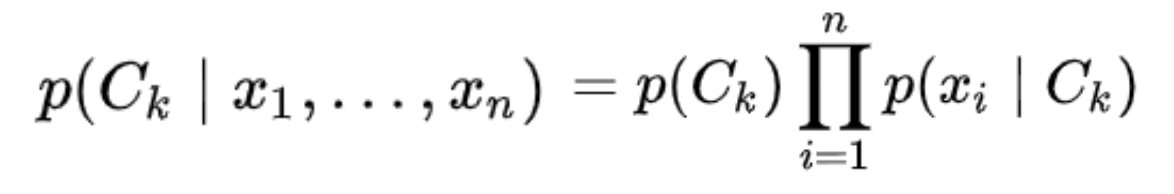
\includegraphics[width=\linewidth]{equation.png}
  \caption{Naive Bayes Classifiers}
  \label{fig:boat1}
\end{figure}

A react webapp was created in order to aid user input and to simulate the results. On load, the network of 20 users was visualized as a series of interconnected nodes. In order to run the simulation, you click a node, enter a potential tweet, then click submit. This tweet is then sent to the backend (which was written in python), the new tweet was broken down into tokens, and then the Naive Bayes Classification formula was run based on occurrences of the words in our simulated tweet within our downloaded history. In deterministic mode, if the value for the positive classifier exceeded the value for the negative classifier, we then considered the user to have retweeted the tweet, and ran the simulation again on each of that user's neighboring nodes. However, since the majority of tweets are not retweeted, this lead to a simulation which only classified tweets as being retweeted if all of the words had a high probability of being in a retweeted tweet. This meant tweets which used lots of common words that were not retweeted, but did in fact appear in tweets that were actually retweeted, were being classified as not retweeted. In order to mitigate this issue and make the simulation more realistic, a non-deterministic mode was added. This mode took the number for the positive classification $C_{positive}$ and the number for the negative classification $C_{negative}$ and made a ratio out of them via the equation $C_{positive}/(C_{positive} + C_{negative})$. If a random value between 0 and 1 was less than or equal to this value, we would consider the tweet retweeted. This lead to more frequent retweet classifications and is believed to be a more realistic simulation.

\section{Results}

The network chosen was primarily centered around tech figures, particularly those with an interest in crypto, so simulating tweets that used keywords like "crypto", "javascript", "blockchain", generally had more positive results than other random tweets attempted. The non deterministic mode seemed much more reasonable than the deterministic mode, as in deterministic mode, many things were not retweeted. If this project were to be further improved, we'd want to incorporate some of the assumptions listed in the beginning as additional variables that we could train on. In addition, we'd probably want to allow the user to get the average chance a certain node was reached in non-deterministic mode so a user could get a sense of what the probability a certain percentage of their network might be hit with any given tweet. This would require running the simulation multiple times, but would be quite doable.

https://github.com/Didericis/twitter-rumor-spreader

\end{document}
